% Created 2023-01-22 Sun 14:32
% Intended LaTeX compiler: xelatex
\documentclass[11pt,twoside,landscape]{article}
\usepackage{graphicx}
\usepackage{longtable}
\usepackage{wrapfig}
\usepackage{rotating}
\usepackage[normalem]{ulem}
\usepackage{amsmath}
\usepackage{amssymb}
\usepackage{capt-of}
\usepackage{hyperref}
\usepackage{subcaption}
\usepackage[newfloat]{minted}
\usepackage{color}
\usepackage{listings}
\usepackage[top=2cm,bottom=2cm,right=2cm,left=2cm,landscape]{geometry}
\usepackage{multicol}
\usepackage{enumitem}
\usepackage{fancyhdr}
\usepackage{caption}
\usepackage{algorithm}
\usepackage{algpseudocode}
\usepackage{float}
\setlist{noitemsep}
\setlength{\parindent}{0pt}
\setlength{\columnseprule}{0.2pt}
\definecolor{mygreen}{rgb}{0,0.6,0}
\definecolor{mygray}{rgb}{0.5,0.5,0.5}
\definecolor{mymauve}{rgb}{0.58,0,0.82}
\lstset{ backgroundcolor=\color{white}, basicstyle=\footnotesize, breaklines=true, captionpos=b, commentstyle=\color{mygreen}, escapeinside={\%*}{*)},keywordstyle=\color{blue}, stringstyle=\color{mymauve},}
\author{Olivier Lischer}
\date{\today}
\title{ComBau Summary}
\hypersetup{
 pdfauthor={Olivier Lischer},
 pdftitle={ComBau Summary},
 pdfkeywords={},
 pdfsubject={},
 pdfcreator={Emacs 27.2 (Org mode 9.5.5)}, 
 pdflang={English}}
\begin{document}

\pagestyle{fancy}
\fancyhf{}
\fancyhead[R]{ComBau-HS22}
\fancyhead[L]{Summary}
\fancyfoot[CE,CO]{\leftmark}
\fancyfoot[R]{\thepage}
\fancyfoot[L]{Olivier Lischer}

\tableofcontents
\newpage

\begin{multicols}{3}
\section{Compiler \& Runtime System}
\label{sec:org1e98381}
\subparagraph{Runtime System} \
\label{sec:org319ef89}
A Runtime System supports the application execution using software and hardware mechanism.
\subparagraph{Architecture} \
\label{sec:org24a86e0}

{
\begin{center}
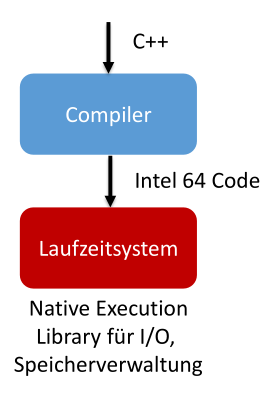
\includegraphics[width=.9\linewidth]{img/cpp_architecutre.png}
\end{center}
\captionof{figure}{C++ Architecture}\label{fig:cpp-architecture}
}


{
\begin{center}
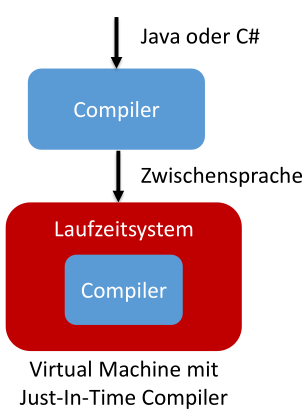
\includegraphics[width=.9\linewidth]{img/java_csharp_architecture.png}
\end{center}
\captionof{figure}{Java / C# Architecture}\label{fig:java-csharp-architecture}
}

{
\begin{center}
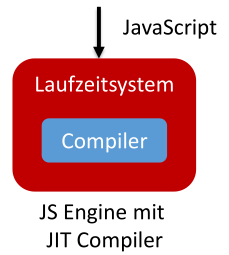
\includegraphics[width=.9\linewidth]{img/js_architecture.png}
\end{center}
\captionof{figure}{JS Architecture}\label{fig:js-architecture}
}

\subparagraph{Compiler Architecture} \
\label{sec:orga5d452c}
A compiler consists of the following parts:
\begin{itemize}
\item Lexer
\item Parser
\item Semantic Checker
\item Optimization
\item Code Generator
\end{itemize}


{
\begin{center}
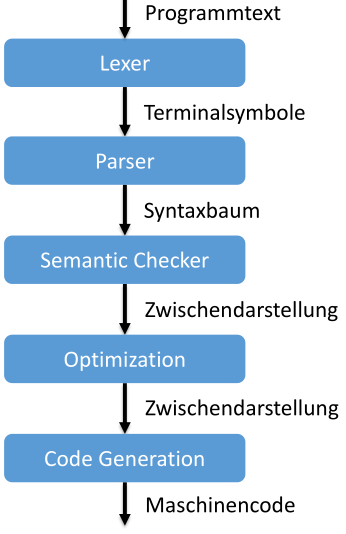
\includegraphics[width=.9\linewidth]{img/compiler_architecture.png}
\end{center}
\captionof{figure}{General Compiler Architecture}\label{fig:general-compiler-architecture}
}

\subparagraph{Runtime Architecture} \
\label{sec:org586795f}
A Runtime System consists of the following parts:
\begin{itemize}
\item Loader
\item Interpreter
\item Metadata, Heap, Stack
\item optional Garbage Collection
\item optional Just-In-Time Compiler
\end{itemize}


{
\begin{center}
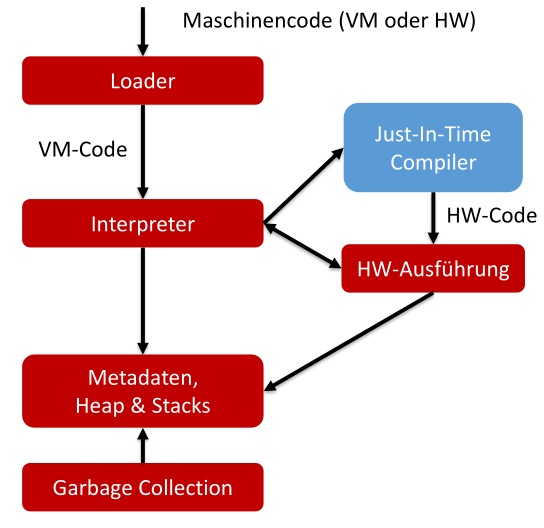
\includegraphics[width=.9\linewidth]{img/runtime_system_architecture.png}
\end{center}
\captionof{figure}{Components of a Runtime System}\label{fig:components-of-a-runtime-system}
}

\subparagraph{EBNF} \
\label{sec:orgffb166d}
The syntax of a language can be expressed using the (E)BNF.
The EBNF has some convenient features but can not express more than the BNF.
\subparagraph{Syntax vs. Semantic} \
\label{sec:orgf7cfb8d}
The syntax defines the structure of the program while the semantic describes the meaning behind the syntax.
The syntax is often described using the \href{../../../roam/20221228120443-how_do_you_specify_the_syntax_of_a_language.org}{EBNF}.
The semantic is often described in prose.
\section{Lexer}
\label{sec:org345a56a}
\subparagraph{Lexer} \
\label{sec:org1c49b9d}
A Lexer takes a string of chars as input (source code) and produces a stream of terminal symbols (tokens).
You want to use a lexer because it will help to parse the input.

{
\begin{center}
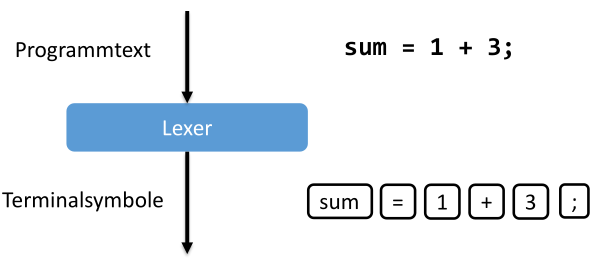
\includegraphics[width=.9\linewidth]{img/lexer_in_output.png}
\end{center}
\captionof{figure}{Input and output from a Lexer}\label{fig:input-and-output-from-a-lexer}
}

A lexer does support only \href{../../../roam/20221228124714-regular_language.org}{Regular Language}.
That means, languages which can expressed using \href{../../../roam/20221228120443-how_do_you_specify_the_syntax_of_a_language.org}{EBNF} without recursion.
Therefore, a look ahead of one char is enough to implement a lexer.

\begin{verbatim}
Integer = Digit { Digit }. // regular
Digit = "0" | ... | "9".

Ausdruck = [ "(" Ausdruck ")" ]. // not regular
\end{verbatim}
\subparagraph{Chomsky Hierarchy} \
\label{sec:org593180d}
The Chomsky Hierarchy describes what is required to read and understand a specific language.
Lexer, Parser and Semantic Checker reads the Language while the \href{../../../roam/20211109182310-deterministic_finite_automaton.org}{DEA}, Push down Automata and Bounded Turing Machine runs the application.

{
\begin{center}
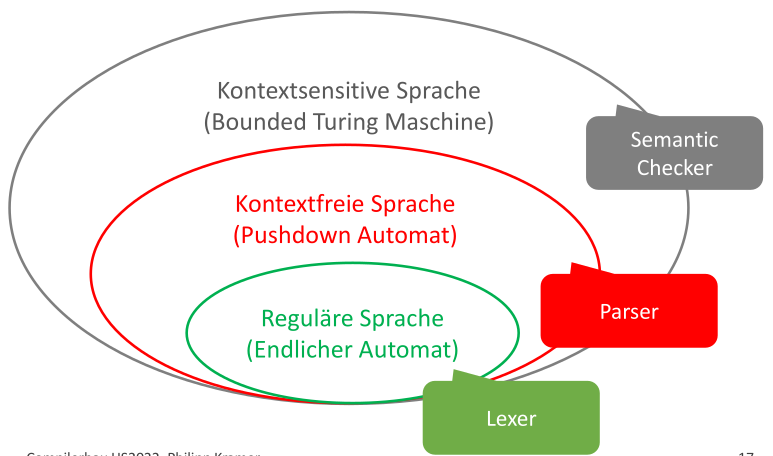
\includegraphics[width=.9\linewidth]{img/chomsky_hierarchie.png}
\end{center}
\captionof{figure}{Chomsky Hierarchy}\label{fig:chomsky-hierarchy}
}

\section{Parser}
\label{sec:org9268a06}
\subparagraph{Parser} \
\label{sec:org5fa0550}
A Parser takes the output of a \href{../../../roam/20221228115248-what_is_a_lexer.org}{Lexer} (token stream) and checks if the input follows the given syntax.
A parser can read only context free languages (see \ref{sec:org593180d}).

The output from a parser is normally an \href{../../../roam/20221228141024-what_is_a_abstract_syntax_tree.org}{Abstract Syntax Tree} or \href{../../../roam/20221228140533-what_is_a_parse_tree.org}{Concrete Syntax Tree}.
If you write the parser by your self you normally want to create an \href{../../../roam/20221228141024-what_is_a_abstract_syntax_tree.org}{AST}.

{
\begin{center}
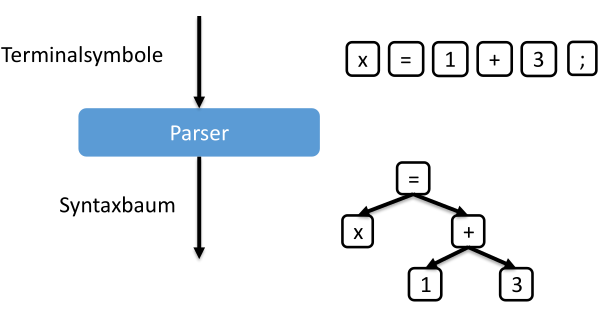
\includegraphics[width=.9\linewidth]{img/parser_in_outputs.png}
\end{center}
\captionof{figure}{In- and Output for Parser}\label{fig:in-and-output-for-parser}
}
\subparagraph{Pare Tree} \
\label{sec:org2022e7e}
A parse tree a.k.a. Concrete Syntax Tree is a derivation of the syntax rules as tree.
A Concrete Syntax Tree contains everything, even the not required parentheses.
The order of the evaluation is implicitly given through the data structure.

The \href{../../../roam/20221228141024-what_is_a_abstract_syntax_tree.org}{Abstract Syntax Tree} is a more minimal version of the Concrete Syntax Tree.

{
\begin{center}
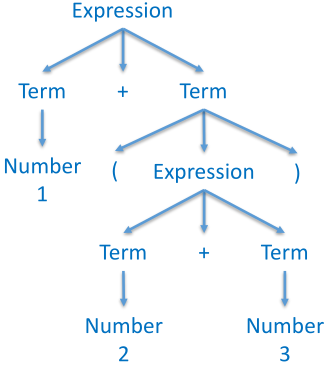
\includegraphics[width=.9\linewidth]{img/concrete_syntax_tree.png}
\end{center}
\captionof{figure}{Concrete Syntax Tree}\label{fig:concrete-syntax-tree}
}

\subparagraph{AST} \
\label{sec:org3ddff65}
The Abstract Syntax Tree is a possible output from the \href{../../../roam/20221228115311-what_is_a_parser.org}{Parser}.
The Abstract Syntax Tree contains only the required information.
For example parentheses are not stored for a \href{../../../roam/20201116150053-java.org}{Java} AST.

\subparagraph{Top-Down Parsing} \
\label{sec:org3d96e2c}
A Top-Down \href{../../../roam/20221228115311-what_is_a_parser.org}{Parser} will start with the Start Symbol form the \href{../../../roam/20221228120443-how_do_you_specify_the_syntax_of_a_language.org}{EBNF} and performs production on the input.
The Top-Down parser will expand from the start symbol to the terminal symbol.

{
\begin{center}
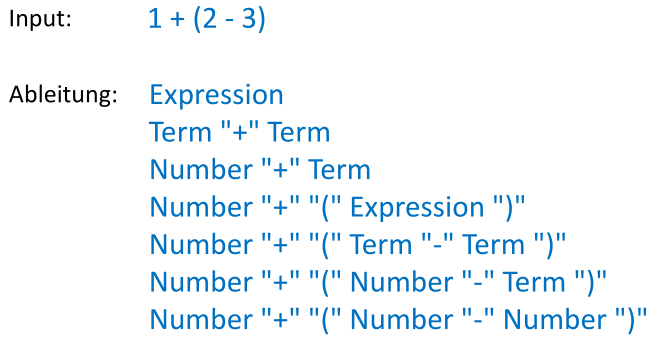
\includegraphics[width=.9\linewidth]{img/top_down_parsing.png}
\end{center}
\captionof{figure}{Top-Down Parsing}\label{fig:top-down-parsing}
}

\subparagraph{Bottom-Up Parsing} \
\label{sec:org68da740}
A Bottom-Up parser starts with the input stream (tokens).
As soon as the parser can match the input on a rule it will reduce it.

{
\begin{center}
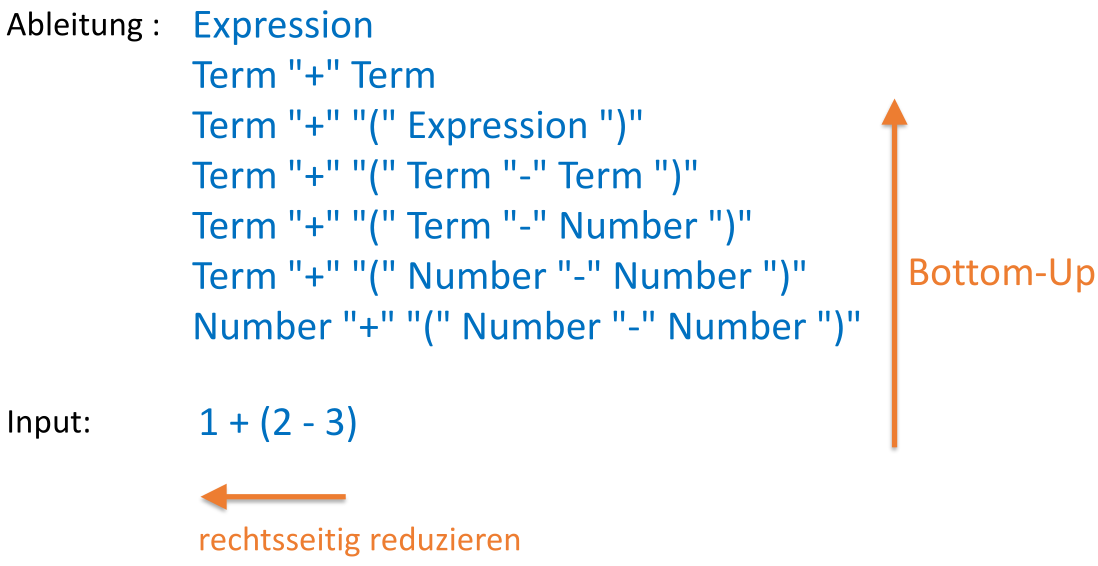
\includegraphics[width=.9\linewidth]{img/bottom_up_parsing.png}
\end{center}
\captionof{figure}{Bottom-Up Parsing}\label{fig:bottom-up-parsing}
}
\subparagraph{Recursive Descent Parser} \
\label{sec:org7008790}
A recursive descent parser is a Top-Down Parser. 
For each non-terminal symbol in a \href{../../../roam/20221228120443-how_do_you_specify_the_syntax_of_a_language.org}{EBNF} you will implement a function.
During parsing, it will call the function \texttt{parseExpression} which will call \texttt{parseTerm}.
The \texttt{parseTerm} function will call again \texttt{parseExpression} (recursion).

The Recursive Descent Parser is a Push-Down Automata which uses the call stack as its stack.

\begin{verbatim}
Expression = Term { ( "+" | "-" ) Term }.
Term = Number | "(" Expression ")".
\end{verbatim}

\begin{lstlisting}[language=java,label= ,caption= ,captionpos=b,numbers=none]
void parseExpression() {
    parseTerm();
    while (is(Tag.PLUS) || is(Tag.MINUS)) {
	next();
	parseTerm();
    }
}

void parseTerm() {
    // ...
    parseExpression();
    // ...
}
\end{lstlisting}
\subparagraph{Parser Categories} \
\label{sec:org617ce08}
\begin{itemize}
\item first letter
\begin{description}
\item[{L}] read from left to right
\item[{R}] read from right to left
\end{description}
\item second letter
\begin{description}
\item[{L}] Left-most expansion (top-down parser)
\item[{R}] right-most reduction (bottom-up parser)
\end{description}
\item number in parentheses
\begin{itemize}
\item number of symbols look ahead
\end{itemize}
\end{itemize}

{
\begin{center}
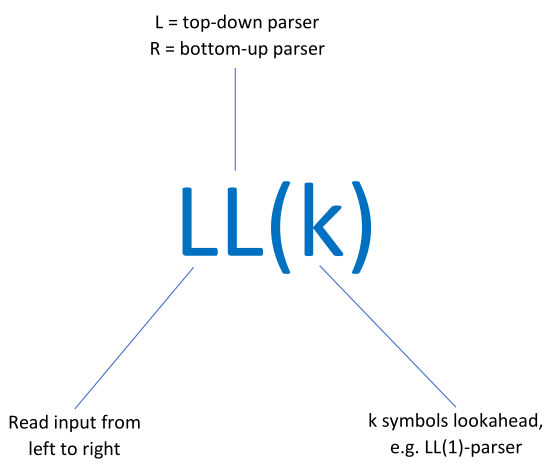
\includegraphics[width=.9\linewidth]{img/parser_notation.png}
\end{center}
\captionof{figure}{Parser notation}\label{fig:parser-notation}
}
\section{Semantic Checker}
\label{sec:org2302e8b}
\subparagraph{Semantic Checker} \
\label{sec:orgded5862}
A Semantic Checker takes the syntax tree (\href{../../../roam/20221228141024-what_is_a_abstract_syntax_tree.org}{AST} / \href{../../../roam/20221228140533-what_is_a_parse_tree.org}{Concrete Syntax Tree}) from the \href{../../../roam/20221228115311-what_is_a_parser.org}{Parser} and returns the syntax tree with a \href{../../../roam/20221229173335-what_is_the_symbol_table_produced_by_a_semantic_checker.org}{Symbol Table}.
The semantic checker performs context-sensitive checks as:
\begin{description}
\item[{declaration}] is every identifier uniquely declared
\item[{types}] are the type rules satisfied
\item[{methoden calls}] are arguments and parameters compatible
\item and more (no cyclic inheritance, single main, \ldots{})
\end{description}


To perform this checks the checker requires all declarations (variables, methods, classes) and all types (predefined, user defined, array, type polymorphism).
\subparagraph{Symbol Table} \
\label{sec:orgde0a275}
The Symbol Table is a data structure produced by the \href{../../../roam/20221228115353-what_is_a_semantic_checker.org}{Semantic Checker}.
The Symbol table is used to manage all declaration in a program source code.

The symbol table contains a mapping from \emph{Symbol} to the \emph{AST} node (\texttt{node = symbolTable.getDeclarationNode(symbol);})


{
\begin{center}
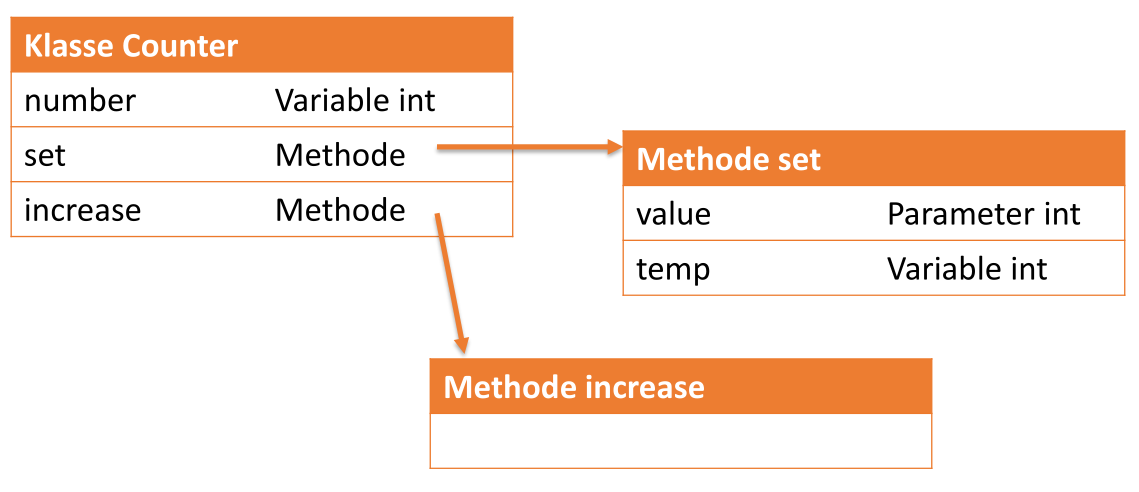
\includegraphics[width=.9\linewidth]{img/symbol_table_example.png}
\end{center}
\captionof{figure}{Example Structure for a Symbol Table}\label{fig:example-structure-for-a-symbol-table}
}

\subparagraph{Symbol Table Construction} \
\label{sec:org3bcf314}
The Semantic Checker performs the following steps:
\begin{enumerate}
\item construct the symbol table
\begin{itemize}
\item traverse AST
\item start with global scope
\item insert symbol in parent scope
\item do not resolve type name and designator yet
\item do not forget Built-in values / types
\end{itemize}

\item resolve all types in table
\begin{itemize}
\item set the type in symbol
\item see \autoref{fig:resolve-types-in-symbol}
\end{itemize}
\item resolve all declarations in \href{../../../roam/20221228141024-what_is_a_abstract_syntax_tree.org}{AST}
\begin{itemize}
\item see \autoref{fig:resolve-declaration-in-ast}
\end{itemize}
\item resolve types in AST
\begin{itemize}
\item set type for each expression
\item see \autoref{fig:resolve-types-in-ast}
\end{itemize}
\end{enumerate}


{
\begin{center}
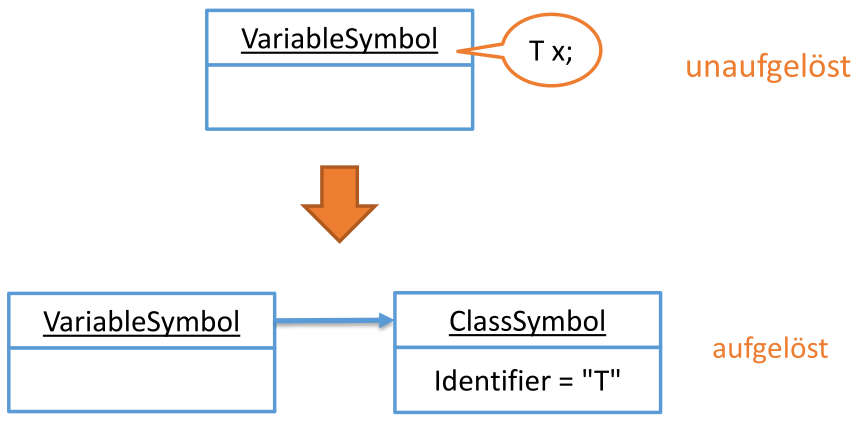
\includegraphics[width=.9\linewidth]{img/resolve_types_in_sybols.png}
\end{center}
\captionof{figure}{Resolve Types in Symbol}\label{fig:resolve-types-in-symbol}
}

{
\begin{center}
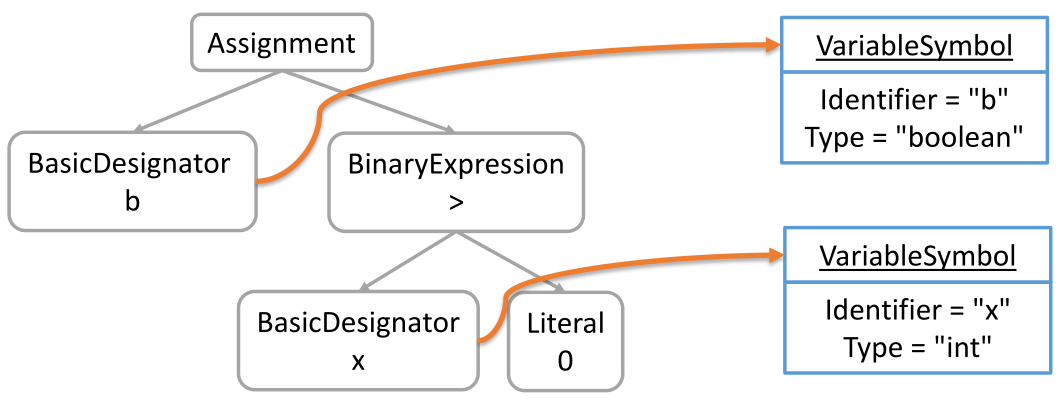
\includegraphics[width=.9\linewidth]{img/resolve_declaration_in_ast.png}
\end{center}
\captionof{figure}{Resolve Declaration in AST}\label{fig:resolve-declaration-in-ast}
}

{
\begin{center}
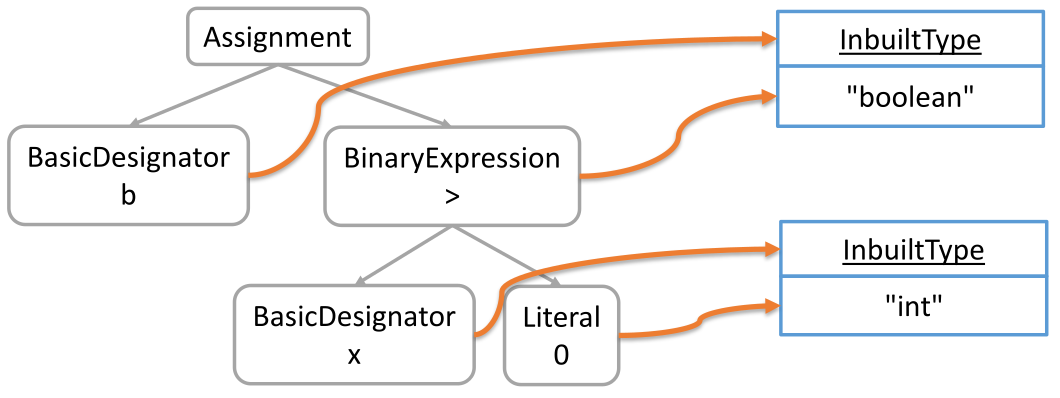
\includegraphics[width=.9\linewidth]{img/resolve_types_in_ast.png}
\end{center}
\captionof{figure}{Resolve Types in AST}\label{fig:resolve-types-in-ast}
}
\section{Code Generation}
\label{sec:org6b399ae}
\subparagraph{Code Generator} \
\label{sec:orgf789d58}
The Code Generator takes the \href{../../../roam/20221229173335-what_is_the_symbol_table_produced_by_a_semantic_checker.org}{Symbol Table} and the \href{../../../roam/20221228141024-what_is_a_abstract_syntax_tree.org}{AST} as input and generates machine code (Intel, ARM, JVM, \ldots{}).
Normally you want to separate the Code Generator from the \href{../../../roam/20221228115311-what_is_a_parser.org}{Parser}, \href{../../../roam/20221228115353-what_is_a_semantic_checker.org}{Semantic Checker}.
If you do so, you can use the same backend to produce code for various different platforms.

{
\begin{center}
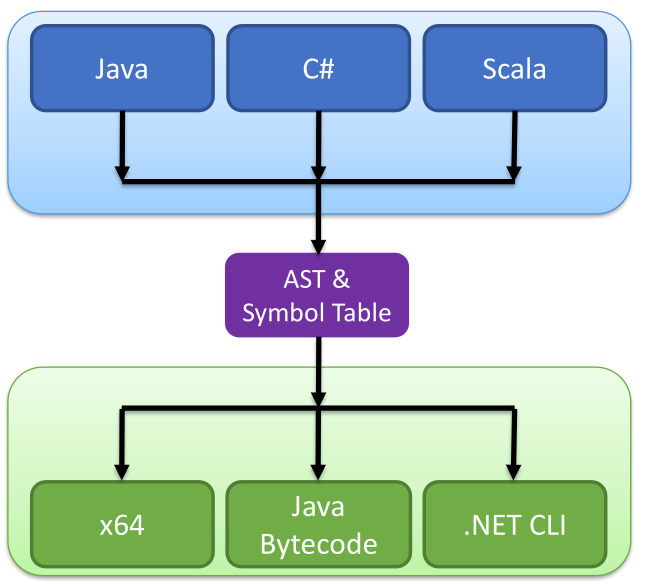
\includegraphics[width=.9\linewidth]{img/backend_ast_frontend.png}
\end{center}
\captionof{figure}{Seperate Backend / Frontend}\label{fig:seperate-backend-frontend}
}
\subparagraph{Evaluation Stack} \
\label{sec:org8b9c731}
In a VM (e.g. JVM - \href{../../../roam/20201116150053-java.org}{Java}) you may use an evaluation stack to run interpret your instructions.
The evaluation stack is an alternative to using registers (what you normally do on real processors).
For example the \texttt{imul} instruction will:
\begin{enumerate}
\item pop y
\item pop x
\item perform z = x * y
\item push z
\end{enumerate}


Each function call has its own evaluation stack and should be empty at the beginning and at the end.


{
\begin{center}
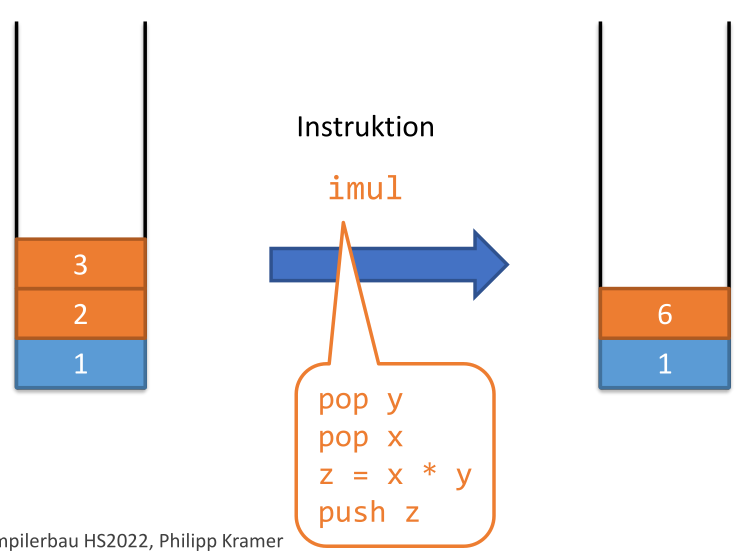
\includegraphics[width=.9\linewidth]{img/eval_stack_imul.png}
\end{center}
\captionof{figure}{Example Evaluation Stack}\label{fig:example-evaluation-stack}
}

\section{Virtual Machine}
\label{sec:orgf09d0ef}
\subparagraph{VM} \
\label{sec:org8eb8d4c}
A VM is a piece of software which emulates a processor.
This processor can have a custom instruction set.

The benefit of a VM is:
\begin{itemize}
\item multiplatform
\item multilanguage (multiple programming languages)
\item security
\end{itemize}


{
\begin{center}
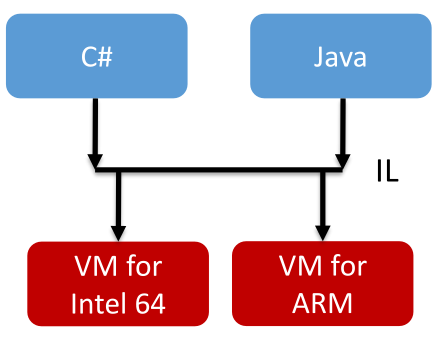
\includegraphics[width=.9\linewidth]{img/vm_example.png}
\end{center}
\captionof{figure}{VM Example}\label{fig:vm-example}
}

\subparagraph{Loader} \
\label{sec:orge92049c}
The loader
\begin{itemize}
\item reads the application binary into memory
\item allocate memory
\item defines memory layout
\item perform address relocation
\item starts program execution
\end{itemize}

\subparagraph{Descriptor} \
\label{sec:orgcc6e486}
A descriptor contains the runtime information for types \& methods:
\begin{itemize}
\item types: classes, arrays or base type
\item classes: field types
\item methods: parameter and local types, return value, byte code
\end{itemize}

\subparagraph{Ancestor Table} \
\label{sec:org1b0192a}
The ancestor table is used to check if a class inherits from another in constant time.
In \autoref{fig:ancestor-table-example} you see an example how such an ancestor table is constructed.
The last element in the table for each class is the reference to itself.
However, this only works for \textbf{Single-Inheritance}.

In languages like \href{../../../roam/20201116150053-java.org}{Java} you don't have to allocate memory for the \texttt{object} class, because every class inherits from it (in the ancestor table this would be -1).

{
\begin{center}
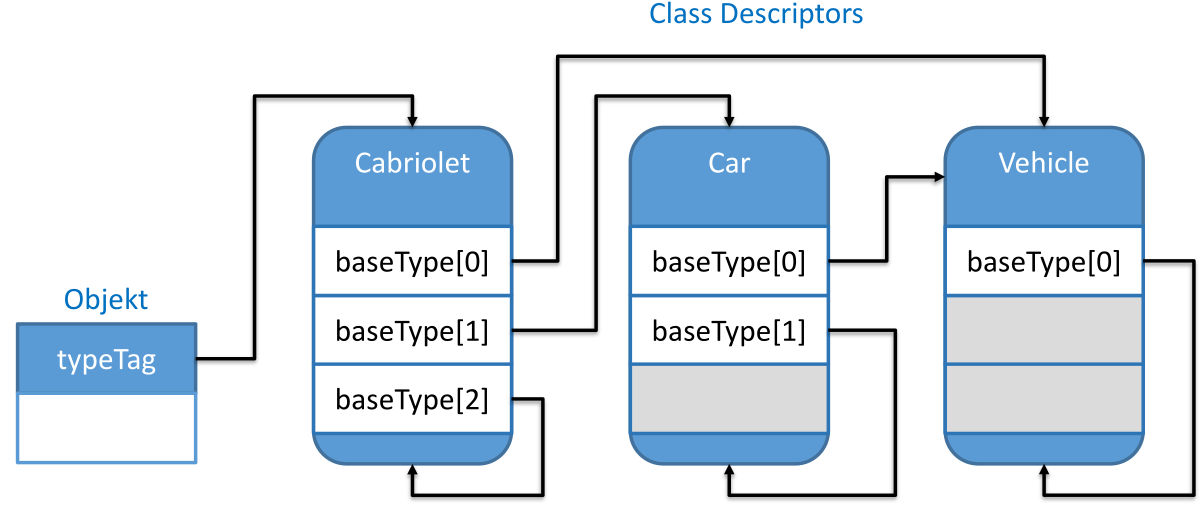
\includegraphics[width=.9\linewidth]{img/ancestor_table.png}
\end{center}
\captionof{figure}{Ancestor Table Example}\label{fig:ancestor-table-example}
}

\subparagraph{Type Cast / Checking} \
\label{sec:org259114f}
You have a target type (you want to cast into this type) and a source type (you want to cast from this type).

\begin{enumerate}
\item Get the ancestor level from the target type (for example 0). Call the level \texttt{x}
\item Check in the ancestor table of the source type if the ancestor at level \texttt{x} is the same as the target class
\end{enumerate}


\begin{lstlisting}[language=java,label= ,caption= ,captionpos=b,numbers=none]
private boolean typeTest(Pointer instance, ClassDescriptor targetType) {
    ClassDescriptor sourceType = heap.getDescriptor(instance);
    if (sourceType == targetType) {
	return true;
    }
    var level = targetClass.getAncestorLevel();

    if (sourceClass.getAncestorTable().length > level) {
	return sourceClass.getAncestorTable()[level] == targetClass;
    } else {
	return false;
    }
}
\end{lstlisting}

\subparagraph{Virtual Table} \
\label{sec:org2fbe653}
Each type has a Virtual Method Table (vtable).
The vtable describes which virtual method should be called when dynamic dispatch is performed. 
In a \href{../../../roam/20221230173400-what_is_a_virtual_machine.org}{VM} the vtable often points not directly to the function but to the method descriptor.

However, this only works with \textbf{Single-Inheritance}.

{
\begin{center}
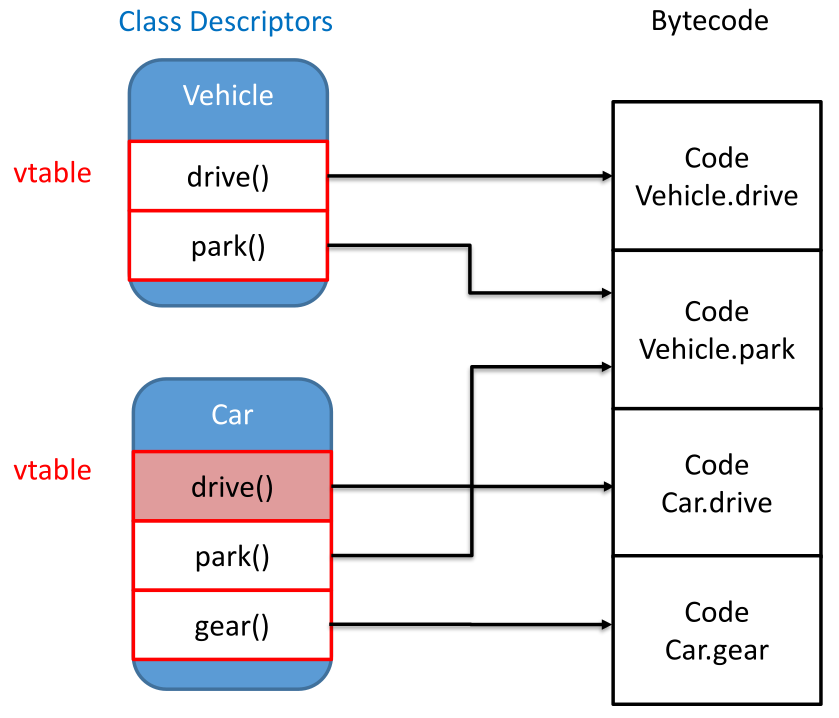
\includegraphics[width=.9\linewidth]{img/vtable_example.png}
\end{center}
\captionof{figure}{VTable example}\label{fig:vtable-example}
}
\subparagraph{Interface Support} \
\label{sec:org73548b5}
To implement dynamic polymorphism using Interfaces you can't use the same approach as using a \href{../../../roam/20221230181314-what_is_the_virtual_method_table.org}{vtable} in inheritance.
Because you would end up with inconsistent numbering (see \autoref{fig:bad-interface-implementation-attempt}).

{
\begin{center}
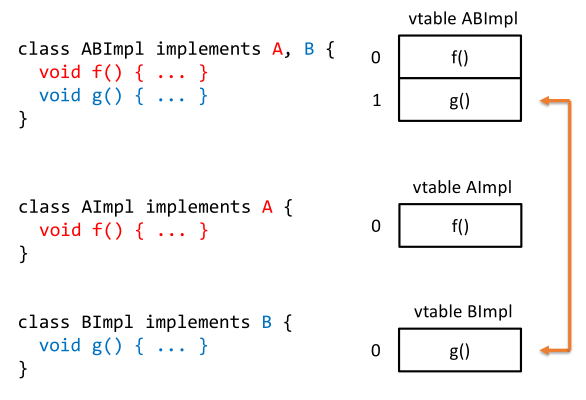
\includegraphics[width=.9\linewidth]{img/interface_bad_attempt.png}
\end{center}
\captionof{figure}{Bad Interface Implementation Attempt}\label{fig:bad-interface-implementation-attempt}
}

To support interfaces you have to globally numbering all interfaces.
For each class you also have to generate an interface table (itable).
This table contains only the implemented interfaces at the same index as they are globally numbered (see \autoref{fig:interface-support}).

{
\begin{center}
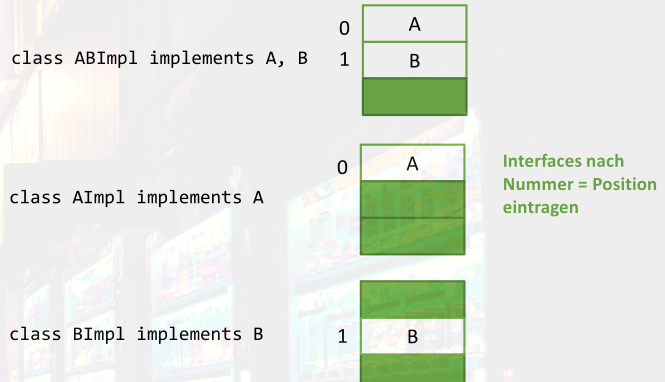
\includegraphics[width=.9\linewidth]{img/interface_support_2.png}
\end{center}
\captionof{figure}{Interface Support}\label{fig:interface-support}
}

To safe memory you can generate a single itable with different offsets.

{
\begin{center}
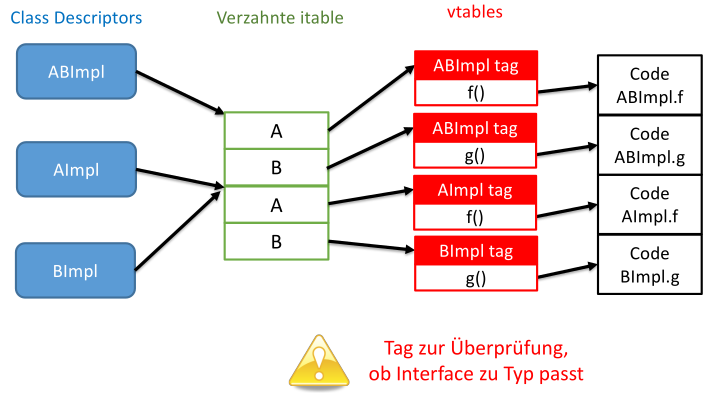
\includegraphics[width=.9\linewidth]{img/total_interface_support.png}
\end{center}
\captionof{figure}{Total Interface Support}\label{fig:total-interface-support}
}

\section{GC}
\label{sec:orgc8dd1bc}
\subparagraph{Dangling Pointer} \
\label{sec:org4c4b0cd}
A dangling pointer is a pointer which points to a location in memory which is already freed.
Reading / Writing to such a pointer can / will cause problems (segfault).

\subparagraph{Memory Leak} \
\label{sec:org539e8fc}
We talk about memory leak if an object is not accessible anymore from the application but are not getting cleaned up.
This is not as dangerous as a \href{../../../roam/20221230183145-what_is_a_dangling_pointer.org}{Dangling Pointer}, but it will fill your memory with useless data.

\subparagraph{GC} \
\label{sec:org60fa478}
The Garbage Collector is a piece of software which automatically cleans unused memory.
The usage of a Garbage Collector is memory safe.
That means:
\begin{itemize}
\item no \href{../../../roam/20221230183145-what_is_a_dangling_pointer.org}{Dangling Pointer}
\item no \href{../../../roam/20221230183215-what_is_a_memory_leak.org}{Memory Leak}
\item an overall simplification for programming
\end{itemize}

\subparagraph{Reference Counting} \
\label{sec:org82bb2f2}
Reference counting is a mechanism to store the number of pointers to a reference.
Every time a pointer starts to point to a resource the counter is incremented.
As soon as one pointer does not point anymore to this location the counter is decremented.

\subparagraph{RC Cyclic Graph} \
\label{sec:org85cb02a}
As soon as you get a cyclic object structure the counter for each object can not reach zero.
Therefore, the Garbage Collector will never recognize it as garbage and a \href{../../../roam/20221230183215-what_is_a_memory_leak.org}{Memory Leak} occurs.


{
\begin{center}
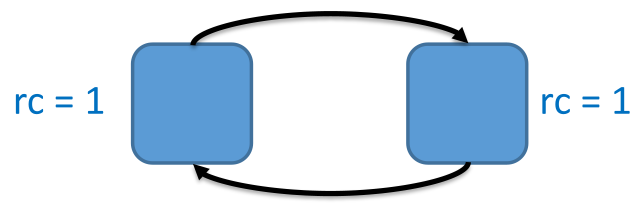
\includegraphics[width=.9\linewidth]{img/cyclic_object_structure.png}
\end{center}
\captionof{figure}{Cyclic Object Structure}\label{fig:cyclic-object-structure}
}

\subparagraph{Mark \& Sweep} \
\label{sec:org0f0915b}
The Mark And Sweep Algorithm can be used to inside a Garbage Collector to find and free garbage.
In the first phase (mark phase) you perform a \href{../../../roam/20220202095038-dfs.org}{DFS} staring from a root set.
Every time you visit a node you mark it.

The root set consists of:
\begin{itemize}
\item all references in static variables
\item all references in all activation frames on the call stack
\item all references in the registers
\end{itemize}

In the second phase (sweep phase) you traverse the whole Heap linearly.
If the node is marked you clear the mark and look at the next node.
If the node is not marked you will free it.


{
\begin{center}
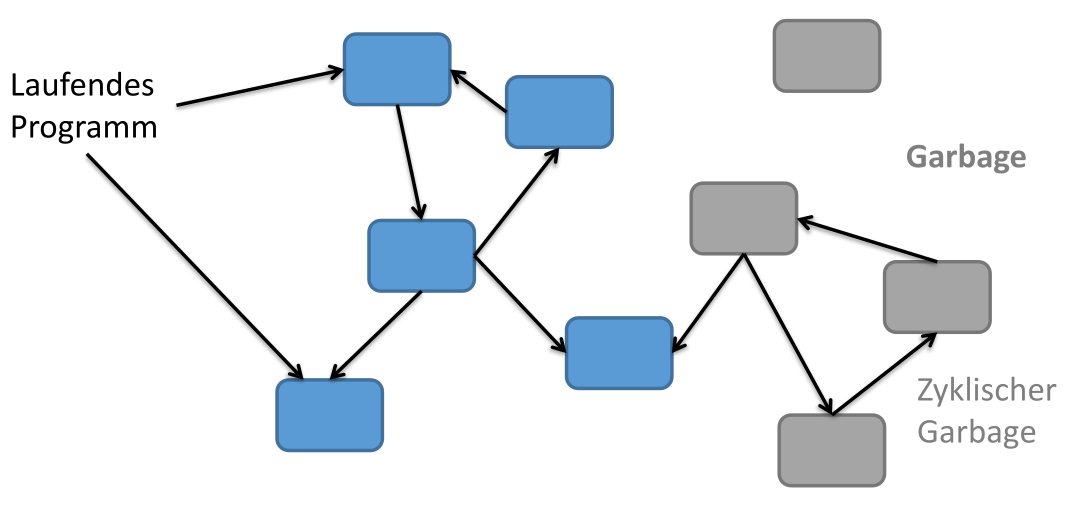
\includegraphics[width=.9\linewidth]{img/heap_graph.png}
\end{center}
\captionof{figure}{Heap Graph of Nodes}\label{fig:heap-graph-of-nodes}
}

\subparagraph{GC Execution} \
\label{sec:orgaf8e3fc}
The Garbage Collector is executed at the latest when the Heap is full.
However, most common Garbage Collector are executed earlier.

Depending on the implementation the application can not run, while the Garbage Collector is working (Stop \& Go).


{
\begin{center}
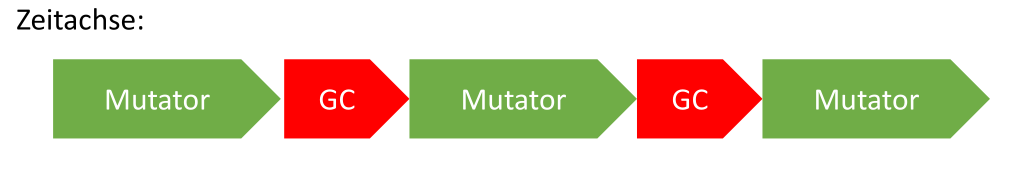
\includegraphics[width=.9\linewidth]{img/stop_and_go_gc.png}
\end{center}
\captionof{figure}{Stop & Go GC}\label{fig:stop-go-gc}
}

\subparagraph{Finalizer} \
\label{sec:org2e848c4}
A Finalizer is a method which is run just before the objects get deleted.
These functions are normally called by the \href{../../../roam/20211008083744-garbage_collection.org}{GC} but not during normal GC phases.

Finalizers are executed in an arbitrary order and time.
They run concurrent to the main program.
In Java the finalizer is \textbf{NOT} executed again after \href{../../../roam/20221231095240-what_is_resurrection.org}{Resurrection}.

\begin{lstlisting}[language=java,label= ,caption= ,captionpos=b,numbers=none]
class Block {
    @Override
    protected void finalize() {
	//...
    }
}
\end{lstlisting}
\subparagraph{Finalizer Execution: Time} \
\label{sec:org62f4b57}
A finalizer is called from the \href{../../../roam/20211008083744-garbage_collection.org}{GC} but not during the normal GC phases. 
Reasons for this are:
\begin{itemize}
\item finalizer might run forever => would block GC
\item finalizer migth create new objects => corrupts GC
\item programming errors in finalizer => GC might crash
\item finalizer can revive objects => \href{../../../roam/20221231095240-what_is_resurrection.org}{Resurrection}
\end{itemize}
\subparagraph{Finalizer Execution: How} \
\label{sec:org8fa97ec}
The \href{../../../roam/20211008083744-garbage_collection.org}{GC} has a \textbf{finalizer set} where all finalizers are registered.
In the \textbf{pending queue} are all finalizers which are not executed yet but has to.
\textbf{Attention}: as soon as you insert the finalizer into the pending queue the object the revived (\href{../../../roam/20221231095240-what_is_resurrection.org}{Resurrection}).
An additional GC phase is required.


{
\begin{center}
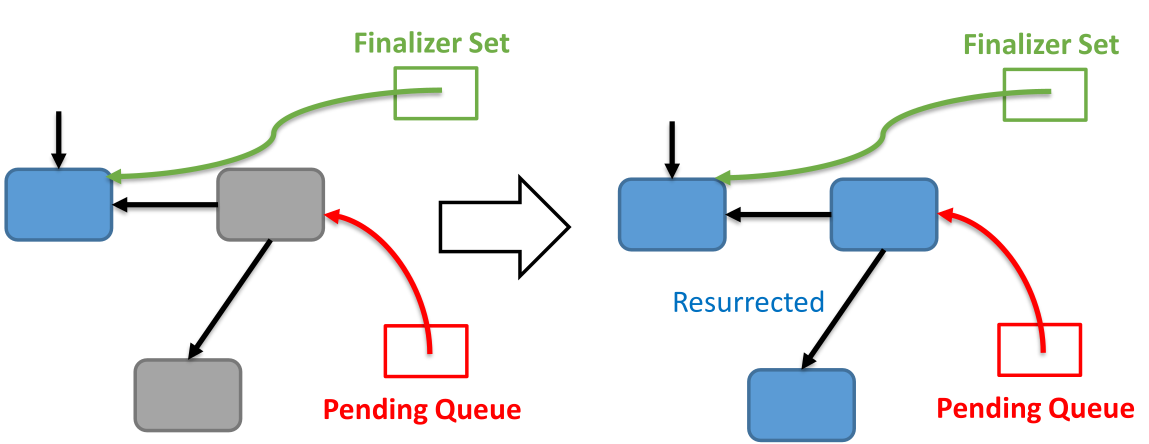
\includegraphics[width=.9\linewidth]{img/pending_queue.png}
\end{center}
\captionof{figure}{Pending Queue}\label{fig:pending-queue}
}
\subparagraph{Resurrection} \
\label{sec:org09772f8}
A finalizer can revive objects (no garbage anymore).
This can happen not only for the current object but also for other objects.


{
\begin{center}
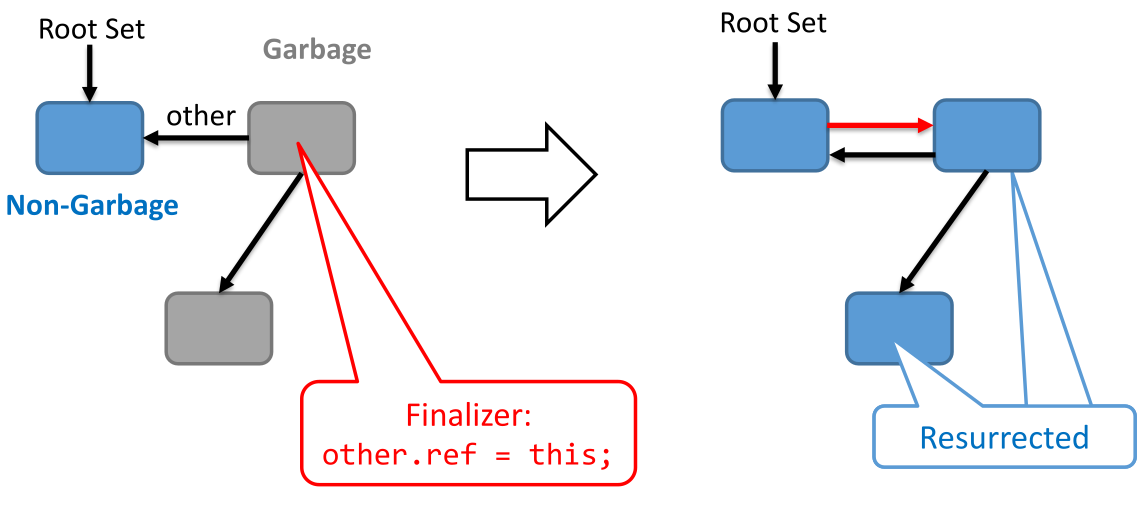
\includegraphics[width=.9\linewidth]{img/resurrection_example.png}
\end{center}
\captionof{figure}{Resurrection Example}\label{fig:resurrection-example}
}
\subparagraph{Weak References} \
\label{sec:org8694543}
A Weak Reference are references which are not counted for Reference Counting.
In a \href{../../../roam/20211008083744-garbage_collection.org}{GC} context this can be used for object caches.
Weak References must be set to \texttt{NULL} after the target object is freed (\href{../../../roam/20221230183145-what_is_a_dangling_pointer.org}{Dangling Pointer}).

{
\begin{center}
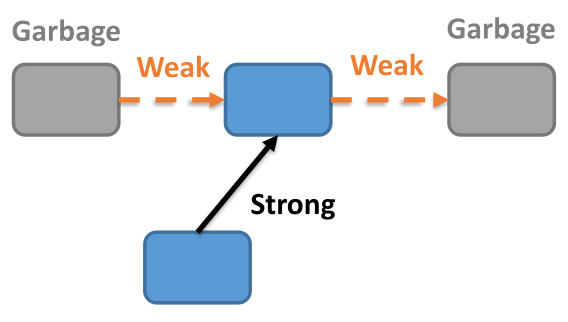
\includegraphics[width=.9\linewidth]{img/weak_reference.png}
\end{center}
\captionof{figure}{Weak Reference Example}\label{fig:weak-reference-example}
}

\subparagraph{Compacting GC} \
\label{sec:orga4fe092}
A compacting GC always allocates at the end of the Heap right after the last object.
During the GC Phases (here mark and copy) the marked objects (non-garbage objects) are copied to the beginning.


{
\begin{center}
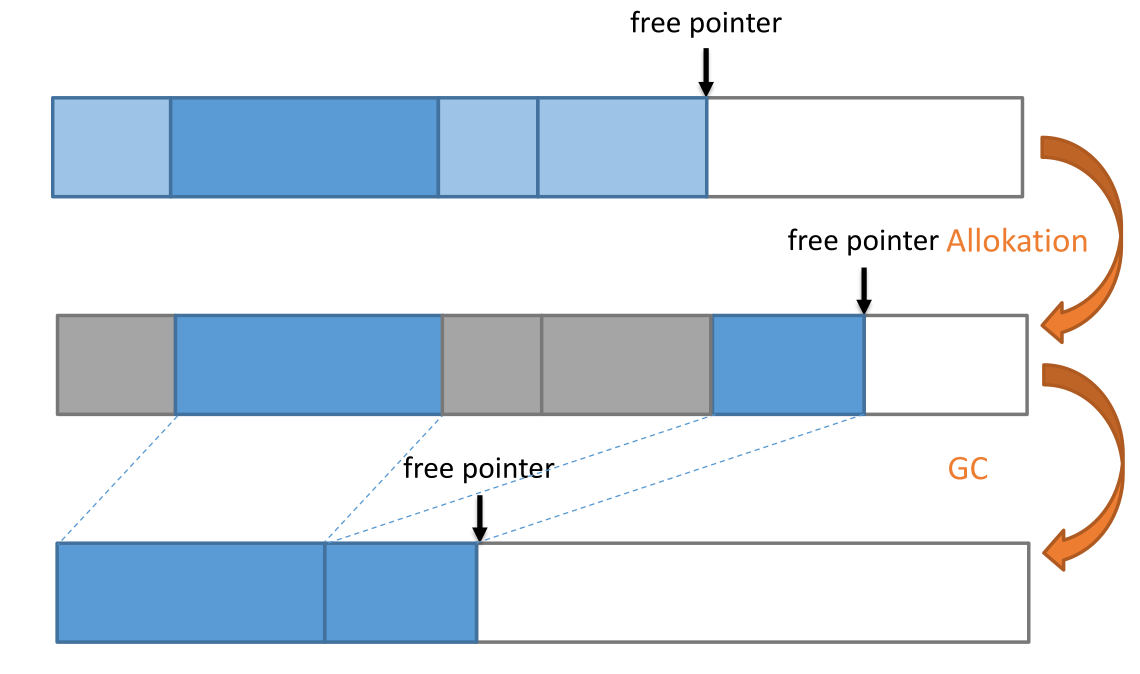
\includegraphics[width=.9\linewidth]{img/compacting_gc.png}
\end{center}
\captionof{figure}{Compacting GC Example}\label{fig:compacting-gc-example}
}
\subparagraph{Incremental GC} \
\label{sec:orgca58502}
An incremental GC runs \textbf{quasi parallel} to the mutator.
The main execution is interrupted only a very short time (No \href{../../../roam/20221230204307-when_is_the_garbage_collector_executed.org}{Stop \& Go GC}).


{
\begin{center}
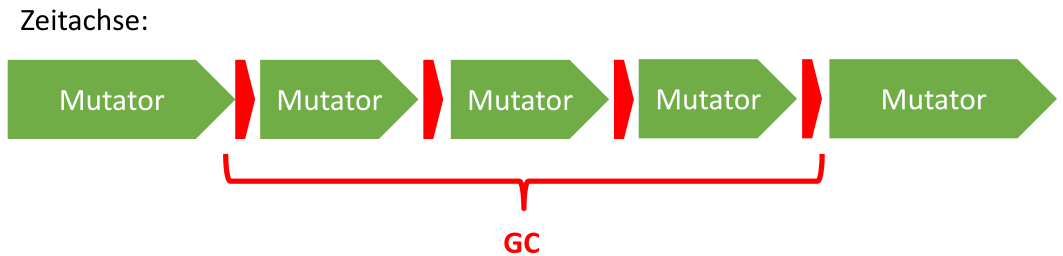
\includegraphics[width=.9\linewidth]{img/incremental_gc.png}
\end{center}
\captionof{figure}{Incremental GC}\label{fig:incremental-gc}
}

\subparagraph{Generational GC} \
\label{sec:org293b444}
A Generational GC is an incremental GC because it often does not clean up the whole heap but in generations.
For example, you have 3 generations as describe in \autoref{tbl:example-for-generations}

{
\begin{center}
\begin{tabular}{llll}
age & generation & GC frequency & GC break\\[0pt]
\hline
new & G0 & high & short\\[0pt]
middle & G1 & middle & middle\\[0pt]
old & G2 & low & long\\[0pt]
\end{tabular}
\end{center}
\captionof{table}{Example for generations}\label{tbl:example-for-generations}
}

If you want to clean up \emph{Gn} you must extend your root set with all references from the latter generations which are pointing into \emph{Gn}.
If you want to clean up \emph{Gn} you also have to clean up all previous generations.

{
\begin{center}
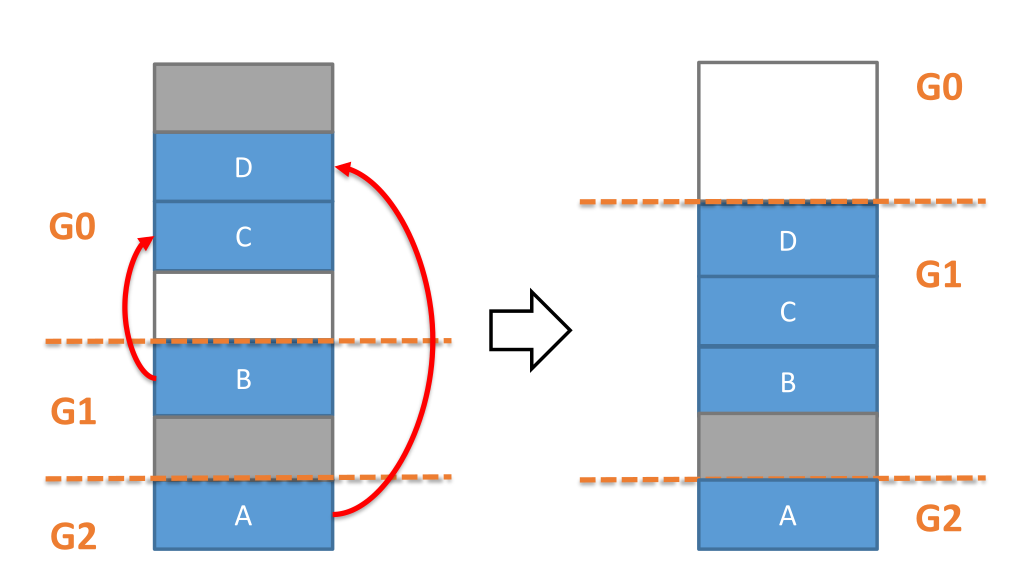
\includegraphics[width=.9\linewidth]{img/gc_of_g0.png}
\end{center}
\captionof{figure}{GC of G0}\label{fig:gc-of-g0}
}

\subparagraph{Partitioned GC} \
\label{sec:orgd24e347}
A Partitioned GC is an incremental GC.
The Heap is partitioned.
The GC will focus on the partition with the most garbage.
The non-garbage objects are moved to a new partition before cleaning up the partition (see \autoref{fig:partitioned-gc}).


{
\begin{center}
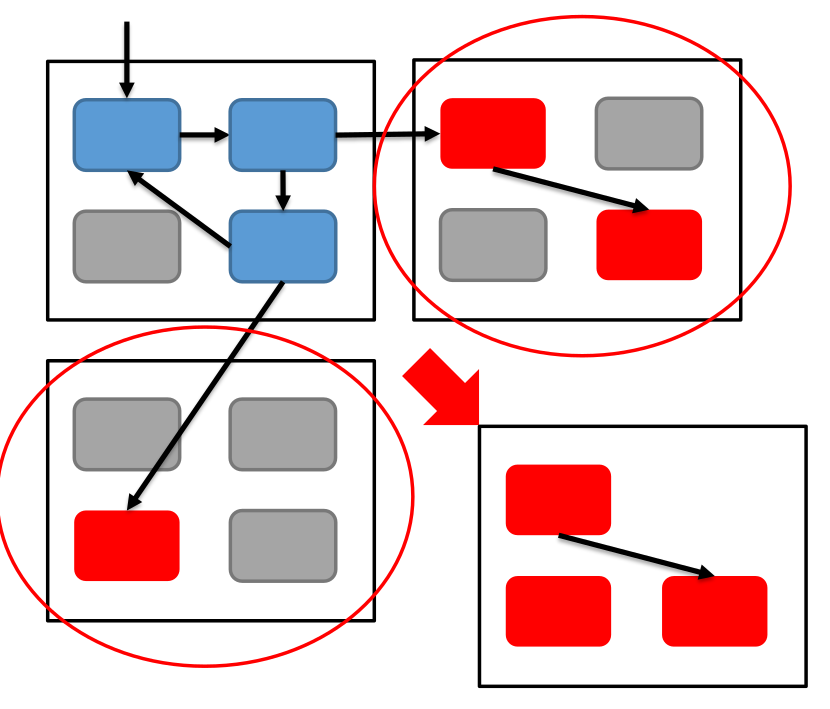
\includegraphics[width=.9\linewidth]{img/partitioned_gc.png}
\end{center}
\captionof{figure}{Partitioned GC}\label{fig:partitioned-gc}
}
\section{JIT}
\label{sec:org44e4e77}
\subparagraph{JIT} \
\label{sec:orgf50a2d2}
A Just-in-Time compiler is used in interpreted languages to compile the intermediate code (e.g. java byte code) to native machine code.
This process speeds up the execution.
Because JIT compiling takes time you normally don't want to compile everything but only so-called \textbf{Hot Spots}.
Hot Spots are code sections which are executed more often.

\subparagraph{Registers} \
\label{sec:org882ddb5}
In the original registers you have to specify another name.
For detail information see \autoref{fig:register-sub-access}.


{
\begin{center}
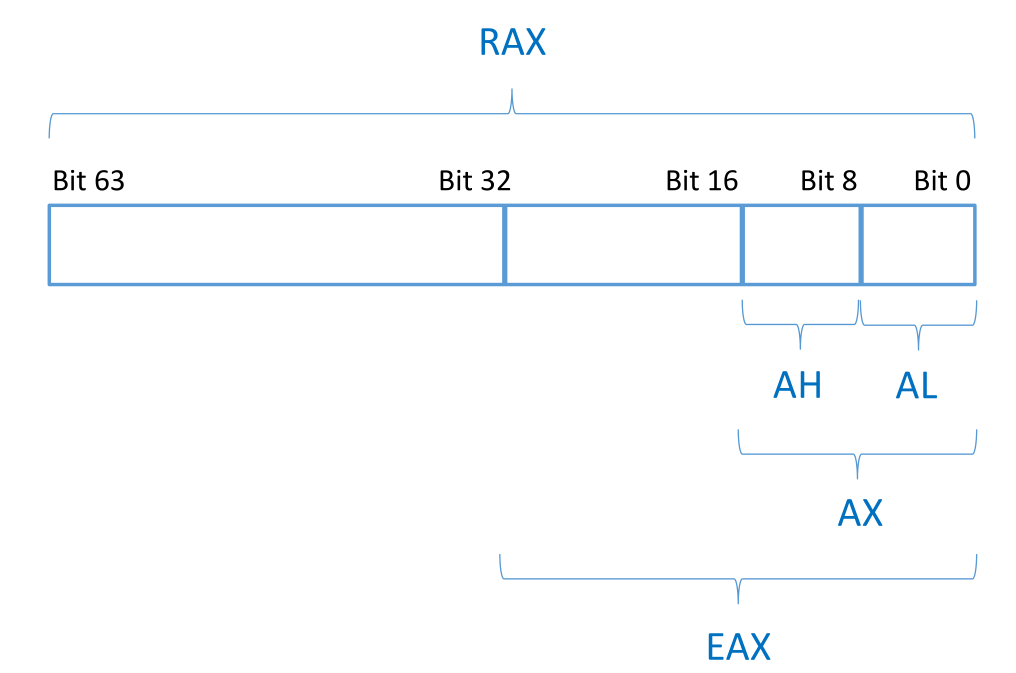
\includegraphics[width=.9\linewidth]{img/register_subaccess.png}
\end{center}
\captionof{figure}{Register sub access}\label{fig:register-sub-access}
}
\subparagraph{Registers Management} \
\label{sec:orgda88f91}
The JIT Compiler keeps track of used registers in a \href{../../../roam/20210806220134-stack.org}{Stack} (similar to the \href{../../../roam/20221230171752-what_is_a_evaluation_stack.org}{Evaluation Stack}).
The stack is updated for each translated byte code instruction.
\subparagraph{Register Clobbering} \
\label{sec:org2a95b23}
For example the \emph{IDVI} assembler instruction overrides the values in \emph{RAX} and \emph{RDX} as side effects.
This is called register clobbering.
Therefore, you have to save thoses values before you executed \emph{IDIV} (Register Relocation).

\subparagraph{Allocation Record} \
\label{sec:org109064e}
The JIT Compiler has to track the usage of the processor registers.
For this you could use the Allocation Record.
The allocation record contains:
\begin{itemize}
\item a list of registers for parameters
\item a list of registers for local variables
\item a set of registers for not used / free registers (missing in \autoref{fig:allocation-record-load-variable})
\item and a linked list / stack for the \href{../../../roam/20221230171752-what_is_a_evaluation_stack.org}{Evaluation Stack}
\end{itemize}


{
\begin{center}
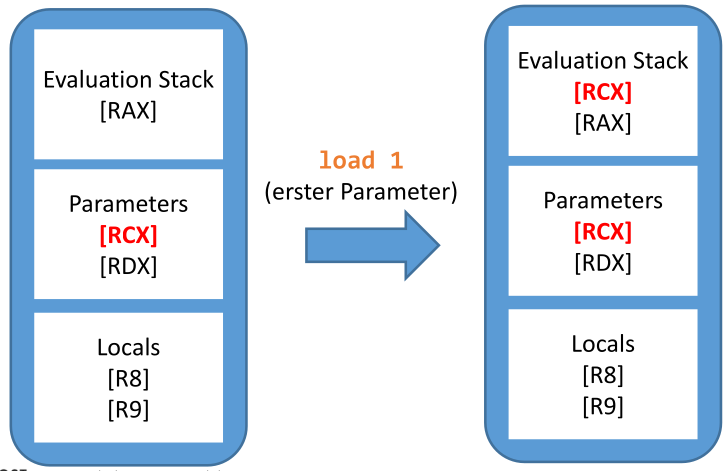
\includegraphics[width=.9\linewidth]{img/allocation_record_load_var.png}
\end{center}
\captionof{figure}{Allocation Record: Load Variable}\label{fig:allocation-record-load-variable}
}
\section{Code Optimization}
\label{sec:orgb55284c}
\subparagraph{Optimizer} \
\label{sec:org1095e11}
The Optimizer is a part of the compiler.
The optimizer transforms an Intermediate Representation or machine code with the goal to generate a more efficient version.
This is often done using multiple steps.
Sometimes the same step is performed multiple times.
\subparagraph{Strategies} \
\label{sec:orgd5a422e}
\begin{itemize}
\item arithmetic optimization
\begin{itemize}
\item replace \texttt{*, /, \%} with bit operations when possible
\end{itemize}
\item algebraic simplification
\begin{itemize}
\item replace const expression with const value
\item \texttt{expr / 1 -> expr}
\item \texttt{expr * 0 -> ldc 0}
\item \texttt{1 + 3 -> ldc 4}
\end{itemize}
\item loop invariant code
\begin{itemize}
\item calculate unchanged expressions during loop outside the loop (see \autoref{lst:loop-invariant} and \autoref{lst:optimizied-loop})
\end{itemize}
\item common sub-expressions
\begin{itemize}
\item calculate same sub-expression only once (var are not allowed to change in between) (see \autoref{lst:common-sub-expression})
\end{itemize}
\item dead code
\begin{itemize}
\item eliminate dead code (May has to be performed multiple times to eliminate all dead code)
\end{itemize}
\item redundant read and write
\begin{itemize}
\item this may lead to dead code elimination
\end{itemize}
\item constant propagation / constant folding
\begin{itemize}
\item some variables are constant even after some long operations
\item load constant, may lead to dead code (in \autoref{lst:constant-propagation} \texttt{ldc 3} has to be performed)
\end{itemize}
\item partial redundancy
\begin{itemize}
\item some expressions are evaluated one or more times (depending on the branching)
\item evaluate only once
\end{itemize}
\end{itemize}


\begin{lstlisting}[language=java,label=lst:loop-invariant,caption={Loop invariant},captionpos=b,numbers=none]
while (x < N * M) { // N * M does never change during loop
  k = y * M;        // k does not change during loop
  x = x + k;
}
\end{lstlisting}


\begin{lstlisting}[language=java,label=lst:optimizied-loop,caption={Optimizied Loop},captionpos=b,numbers=none]
k = y * M;
temp = N * M;
while (x < temp) {
  x = x + k;
}
\end{lstlisting}


\begin{lstlisting}[language=java,label=lst:common-sub-expression,caption={Common sub-expression},captionpos=b,numbers=none]
x = a * b + c;
// operations, but no changes on a and b
y = a * b + d;

temp = a * b;
x = temp + c;
// operations, but no changes on a and b
y = temp + d;
\end{lstlisting}

\begin{lstlisting}[language=java,label=lst:constant-propagation,caption={Constant Propagation},captionpos=b,numbers=none]
a = 1;
if (...) {
    a = a + 1; // a = 2
    b = a;     // b = 2
} else {
    b = 2;
}
c = b + 1;    // c = 2
\end{lstlisting}
\subparagraph{SSA} \
\label{sec:org0afdbbd}
Static Single Assignment is a method to detect optimization possibilities.
In SSA each variable is assigned only once.
If a variable is assigned multiple times you rename it.
Assignments in different branches also get different indexes.
To find the right index at the \href{../../../roam/20230120100519-what_is_the_phi_function_in_ssa.org}{Phi Function} is used.

\begin{lstlisting}[language=java,label=lst:ssa-with-branches,caption={SSA with branches},captionpos=b,numbers=none]
if (...) {
    x_1 = 1;
} else {
    x_2 = 2;
}
y_1 = x_?;
\end{lstlisting}
\subparagraph{Phi Function} \
\label{sec:org85127d8}
The Phi Function is used to check which \texttt{x} should be used during SSA after branching.
In \autoref{lst:phi-function} the phi function performs the following:
\begin{itemize}
\item return \texttt{x\_1} if the \texttt{if} branch was taken
\item return \texttt{x\_2} if the \texttt{else} branch was taken
\end{itemize}

\begin{lstlisting}[language=java,label=lst:phi-function,caption={Phi-Function},captionpos=b,numbers=none]
if (...) {
    x_1 = 1;
} else {
    x_2 = 2;
}
y_1 = phi(x_1, x_2);
\end{lstlisting}
\subparagraph{SSA and Common Subexpression} \
\label{sec:org7e651e3}
Using SSA you can detect multiple assignments to the same variable (or the absence of them).
Thanks to this, you can detect common sub-expressions.

\begin{lstlisting}[language=java,label=lst:common-sub-expressions-in-ssa,caption={Common sub-expressions in SSA},captionpos=b,numbers=none]
x_1 = a_1 * b_1 + c_1;
// some operations
y_1 = a_1 * b_1 + d_1; // no changes on a and b otherwise index would be incremented
// some operations
z = a_1 * b_2 + d_3;
\end{lstlisting}
\subparagraph{SSA and Dead Code} \
\label{sec:org0fbf090}
Thanks to SSA you can detect that \texttt{x\_1} is never read.
Therefore, you don't have to generate code for this expression.

\begin{lstlisting}[language=java,label=lst:dead-code-detection,caption={Dead code detection},captionpos=b,numbers=none]
x_1 = 1;
x_2 = 2;
y_1 = x_2 + 1;
writeInt(y_1);
\end{lstlisting}
\subparagraph{Peephole Optimization} \
\label{sec:orgb6eef76}
Peephole Optimization is used only on a small set of instruction.
This set of instruction is changed using a Sliding Window.
The Optimizations are performed on the sliding window.


{
\begin{center}
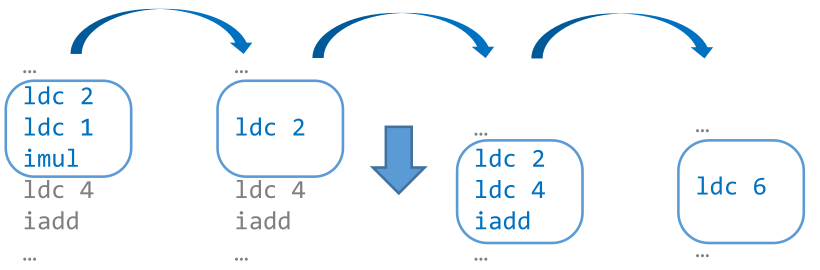
\includegraphics[width=.9\linewidth]{img/peephole_optimization.png}
\end{center}
\captionof{figure}{Peephole Optimization Example}\label{fig:peephole-optimization-example}
}

\section{END}
\label{sec:org98cc237}
\end{multicols}
\end{document}